На момент начала разработки и реализации плагина уже был разработан интерфейс ML модели. Задачей плагина было использование данной ему ML модели для того, чтобы рекомендовать пользователю файлы для модификации, если таковые выдала ML модель.
\section{Плагин GitAlso}
Первой реализацией задачи был GitAlso плагин для IntelliJ платформы. Принцип работы плагина заключался в том, чтобы при пользовательском коммите останавливать процесс сохранения изменений и предложить отменить коммит и модифицировать <<забытые>> файлы.
\subsection{Архитектура}
\begin{figure}[!h]
\caption{Схема архитектуры плагина GitAlso}\label{GitAlso-arch}
\centering
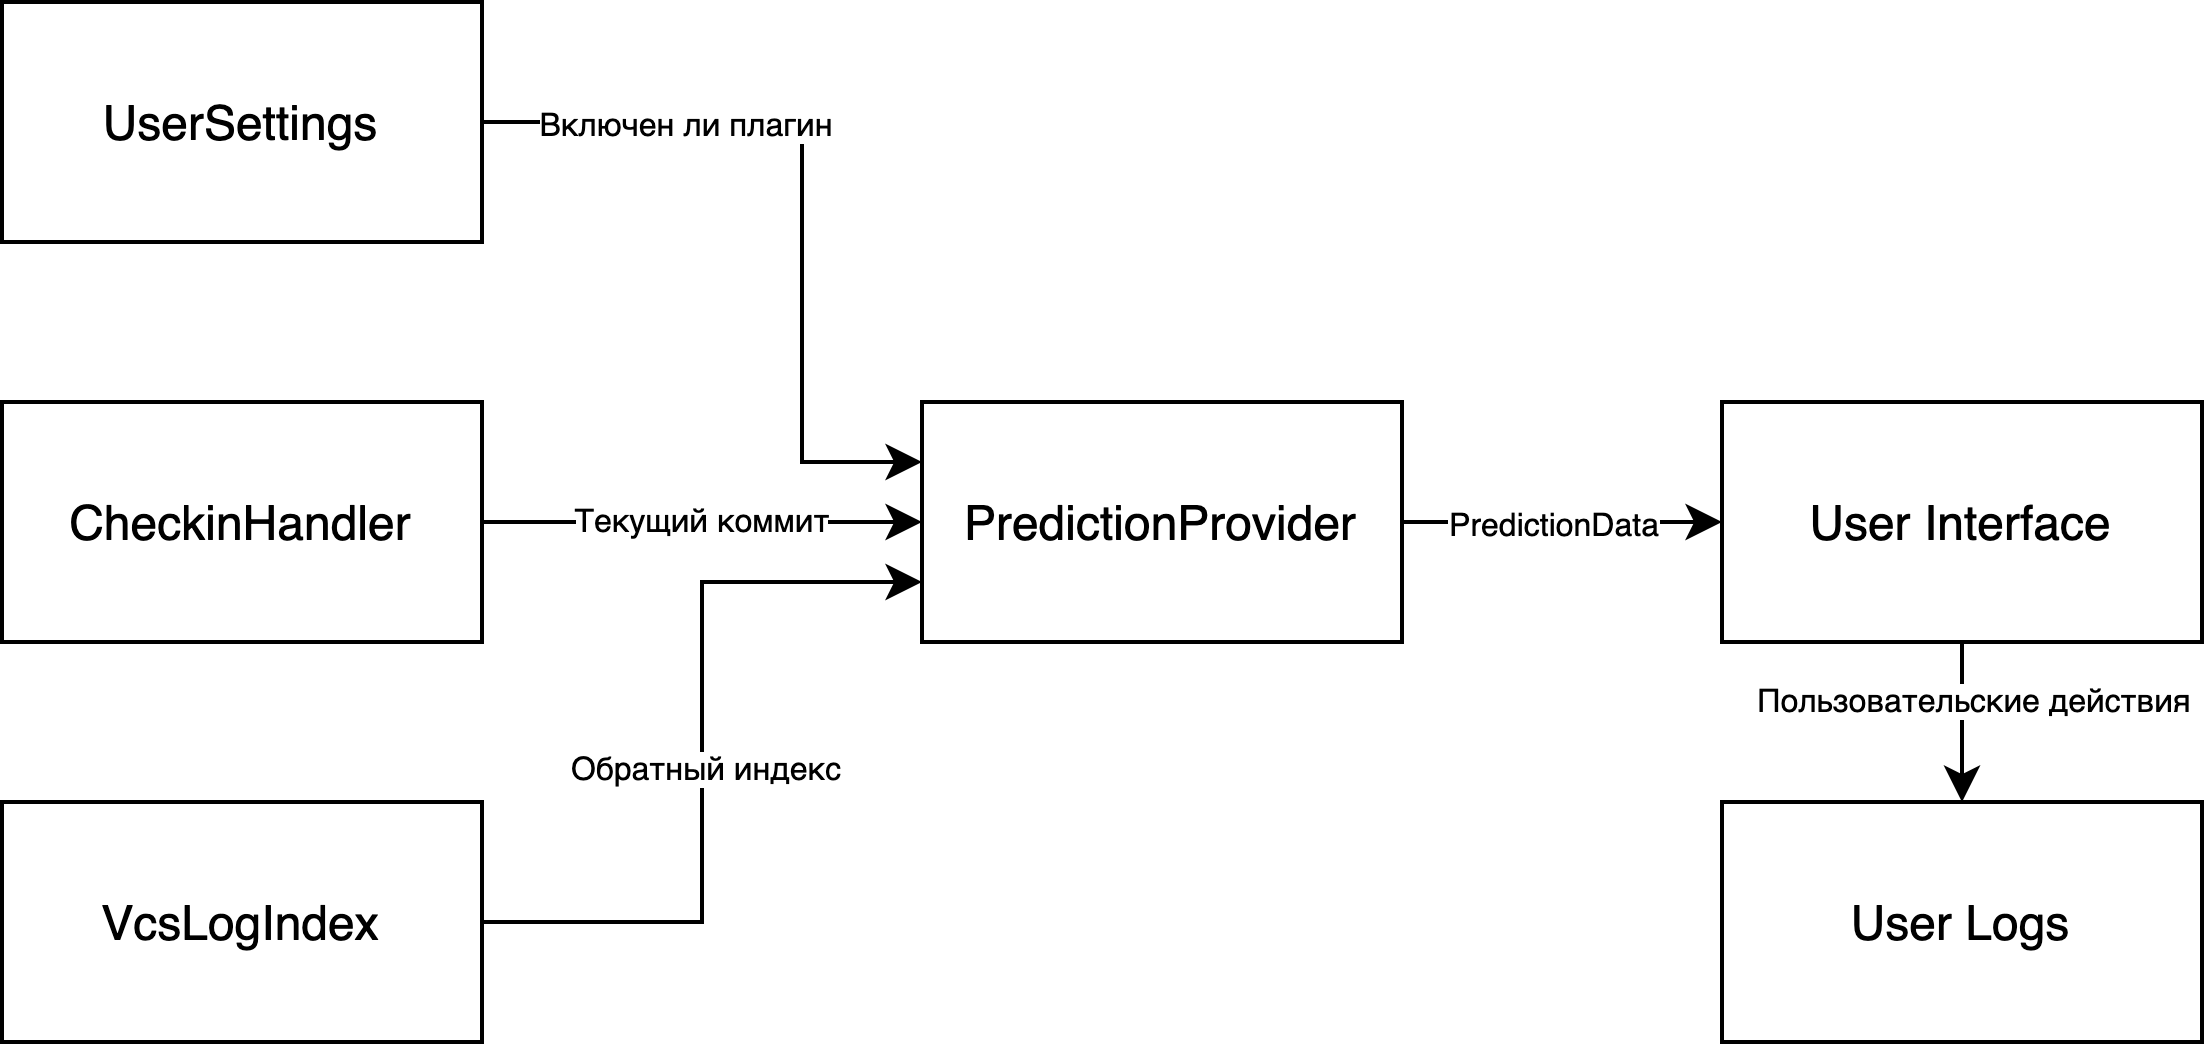
\includegraphics[scale=0.16]{GitAlsoArch.png}
\end{figure}
В IntelliJ платформе, а именно в VCS (Version Control System) части платформы уже был реализован интерфейс для создания так называемых хуков (в платформе они называются $CheckinHandler$). Хук имеет доступ к мета-информации о коммите и файлах, которые должны быть сохранены в репозиторий. Для того, чтобы ML модель выдала рекомендацию следует в дополнение к имеющейся информации получить историю этого самого репозитория в виде множества коммитов (ожидается, что эти коммиты будут связанными). Для получения такой истории нам нужно по заданному набору файлов получить коммиты, в которых эти самые файлы присутствовали. В условиях ограничения по времени отправка и получение такого запроса в Git невозможна, но в Git4Idea плагине для IntelliJ платформе, который идет в комплекте со многими IDE от компании JetBrains и Android Studio, уже присутствуют обратные индексы для коммитов. Значит по данным файлам мы можем быстро узнать идентификаторы коммитов, в которых эти файлы присутствовали. Но одних идентификаторов коммитов нам не достаточно, нам нужны для каждого коммита мета-данные и файлы, которые сохранялись в данном коммите. О получении информации о коммите по индексу будет рассказано в \ref{forward-index}. Таким образом, при создании пользователем коммита создается $CheckinHandler$, который проверяет, создан ли обратный индекс для репозиториев, в которых осуществляется коммит. Если обратный индекс создан, то мы получаем данные, нужные для ML модели и отдаем их в эту модель. Следует обратить внимание, что создание $CheckinHandler$ и вызов методов у него осуществляется на EDT потоке, значит, если подсчет рекомендации будет занимать длительное время, то пользовательский интерфейс будет не доступен долгое время. Чтобы этого избежать, будем выполнять все подсчеты в фоновом процессе, показывая прогресс. После подсчета предсказания будет обновлен пользовательский интерфейс, как будет описано в \ref{git-also-ui}, и собрана статистика, как рассказано в \ref{stats-main}.
\subsection{Прямой индекс}\label{forward-index}
Важным моментом в реализации плагина является получение информации о коммитах из репозитория. Нашему приложению необходимо уметь по данному множеству идентификаторов коммитов возвращать их мета-информацию и файлы, которые в них изменялись. Для выполнения поставленной задачи автором работы был реализован прямой индекс. Его основной положительной стороной является быстрое получение информации о коммите по идентификатору данного коммита, притом реализованный прямой индекс умеет отслеживать переименования файлов. Но реализованный прямой индекс на больших репозиториях занимал существенное количество места на диске. Для репозитория intellij-community на 20 декабря 2019 года прямой индекс занимал 400 мегабайт на жестком диске. Поэтому, было решено использовать запрос в Git для получения информации о коммите по его идентификатору и не учитывать эту часть при подсчете времени подсчета рекомендации, если оно не превышает пяти секунд.
\subsection{Пользовательский интерфейс}\label{git-also-ui}
\begin{figure}[!h]
\caption{Пользовательский интерфейс плагина GitAlso}\label{git-also-screen}
\centering
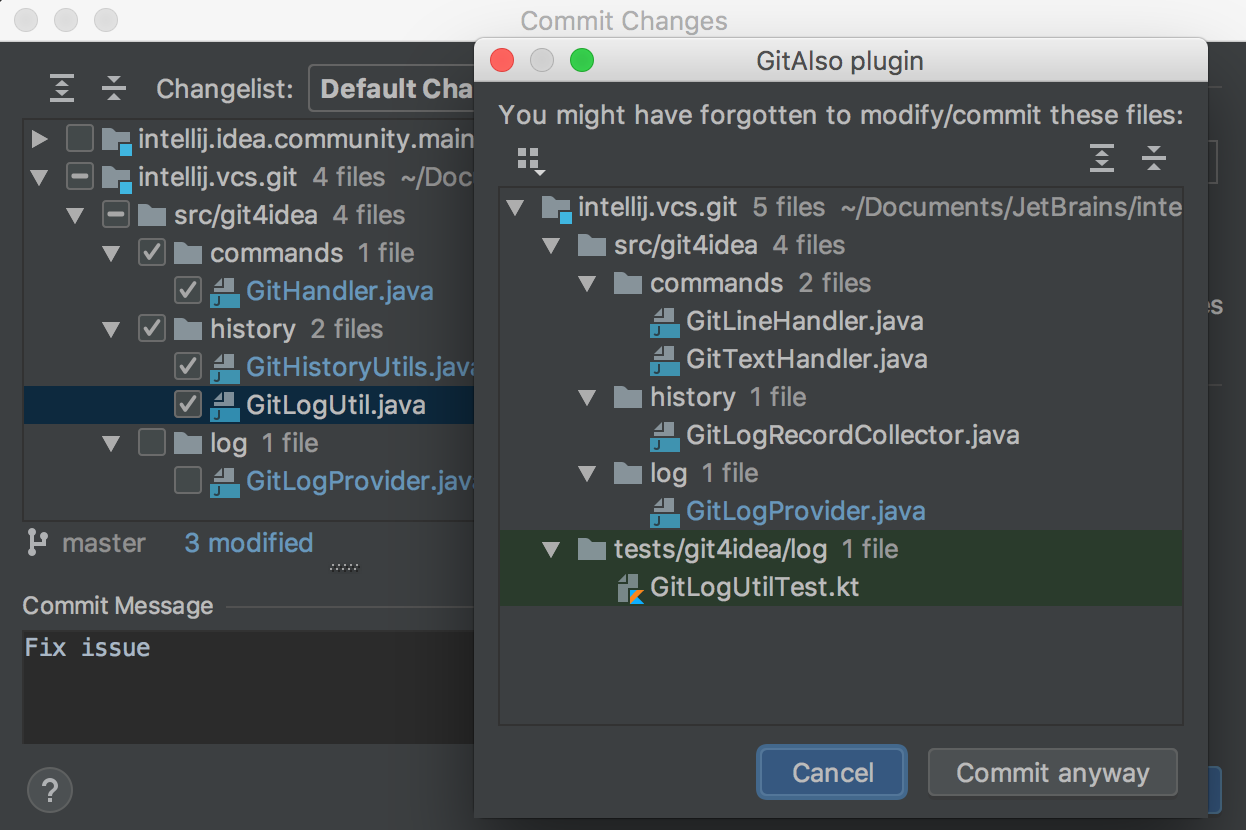
\includegraphics[scale=0.6]{GitAlso.png}
\end{figure}
Пользовательский интерфейс плагина должен показывать файлы, который пользователь возможно <<забыл>> изменить. Для показа таких файлов было решено открывать диалог с деревом файлов. Для показа дерева файлов использовалось готовое решение, которое называется $ChangesBrowser$. Пример показа рекомендации можно увидеть на рисунке  \ref{git-also-screen}.
\subsection{Персонализация решающей функции}
Для улучшения качества показываемых рекомендаций было принято решение использовать взаимодействие пользователя с плагином в целях изменения границы срабатывания решающей функции. На основе нажатий пользователем кнопок Commit Anyway и Cancel мы будем обновлять границу, используя метод $updateState$ приведенный в листинге \ref{personalization}, и сохранять ее в локальное состояние.
\section{Плагин ChangeReminder}
Исходя из результатов анализа статистики собранной в пункте \ref{jet-stat-logs} и анализа в пункте полученной статистики
 %TODO%
, а также отзывов внутри компании, стало понятно, что пользовательский интерфейс плагина GitAlso представленный в пункте \ref{git-also-ui} нужно изменить, избавившись от модальности. Тогда автором работы было принято решение переместить функциональность плагина GitAlso из коммит хука во вкладку Local Changes. В приведенной вкладке показаны файлы, который пользователь модифицировал, добавил, удалил из системы контроля версии. Представим, что пользователь будет сохранять в репозиторий все файлы, которые расположены в его списке изменений по умолчанию. Будем делать рекомендации для данных файлов при каждом их изменении и при изменении репозитория. В связи с такими изменениями было решено создать новый плагин и назвать его ChangeReminder. По большей части функциональность плагина основана на плагине GitAlso, но есть и существенные изменения в архитектуре.
\subsection{Конвертация модели случайного леса в Java код}
\subsection{Архитектура}
\begin{figure}[!h]
\caption{Схема архитектуры плагина ChangeReminder}\label{ChangeReminder-arch}
\centering
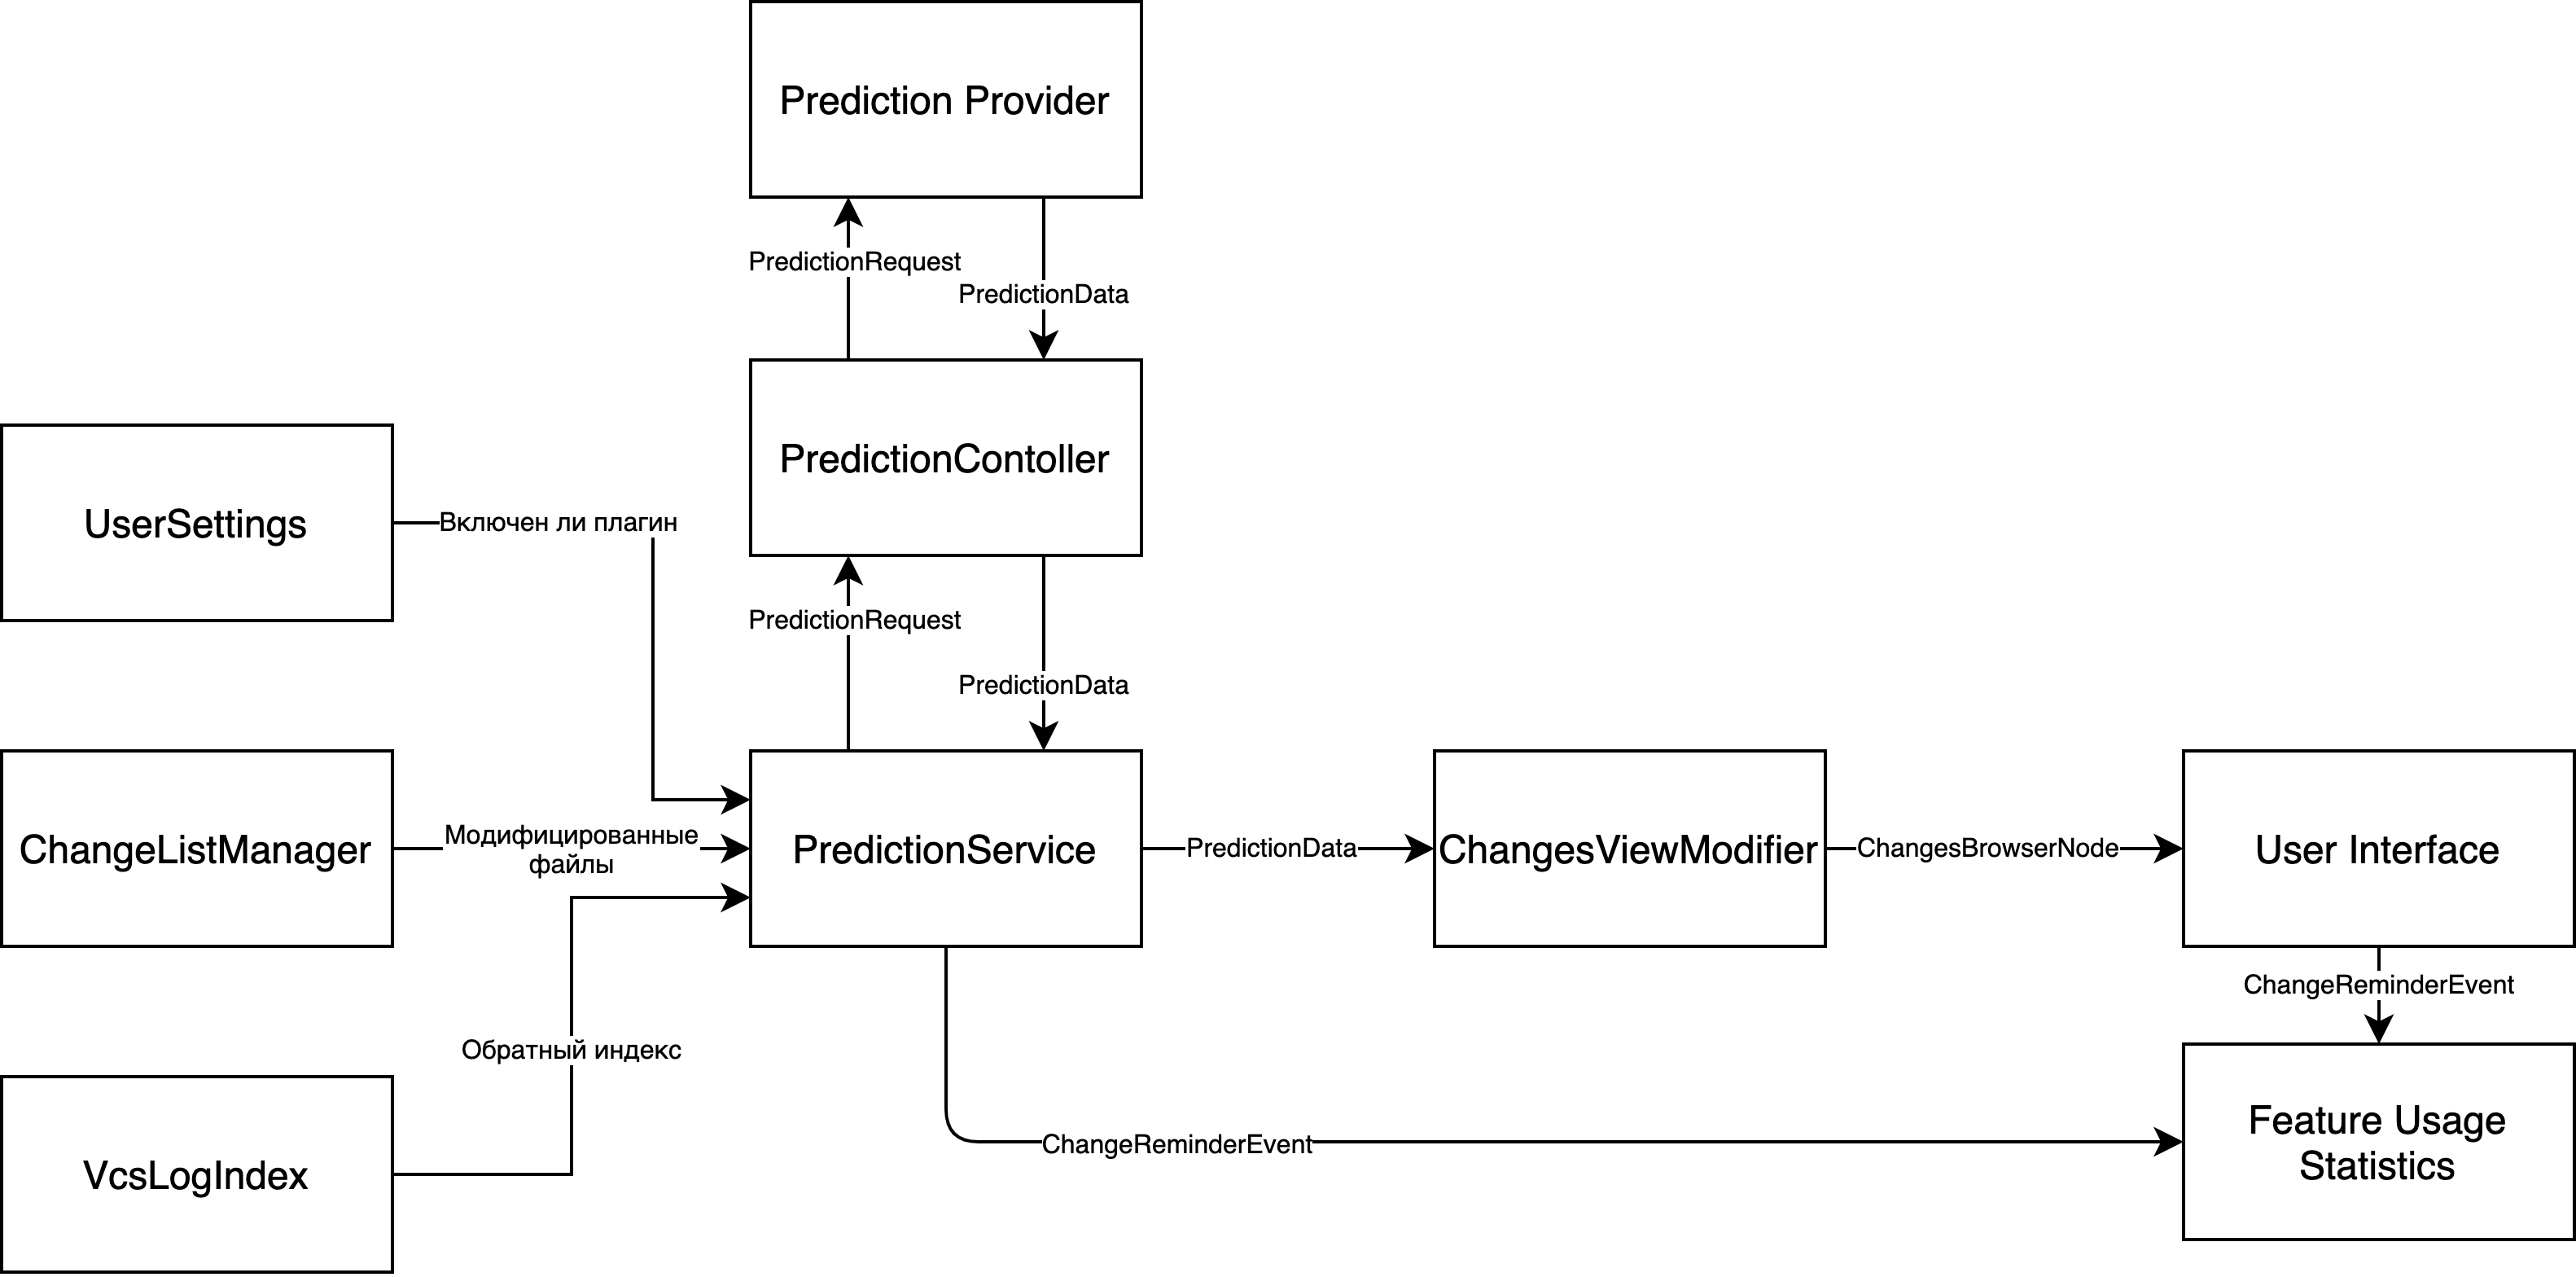
\includegraphics[scale=0.14]{ChangeReminderArch.png}
\end{figure}
Рекомендация файлов пользователю происходит по следующему алгоритму:
    \begin{itemize}[label={\textbullet}]
        \item Пользователь модифицирует файл/изменяется состояние одного из репозиториев.
        \item $ChangeListManager$ сообщает в $PredictionService$ о том, что список изменений по умолчанию изменился.
        \item $PredictionService$ запрашивает у $UserSettings$ включен ли плагин, если нет, то дальнейшие действия не происходят.
        \item $PredictionService$ запрашивает у $VcsLogIndex$ обратный индекс для текущих репозиториев, если индекс еще не готов, то дальнейшие действия не происходят.
        \item $PredictionService$ отправляет $PredictionRequest$ на обработку в $PredictionController$.
        \item $PredictionController$ занимается обработкой запроса и отдает $PredictionData$~-- результат работы в $PredictionService$
        \item $PredictionService$ запрашивает обновление у $ChangesViewModifier$
        \item $ChangesViewModifier$ из данной $PredictionData$ создает $ChangesBrowserNode$, которая рисуется в пользовательстком интерфейсе.
    \end{itemize}
$PredictionService$ и действия пользователя с интерфейсом записываются в сервисе Feature Usage Statistics (см. пункт \ref{fus-main}). Описанный выше алгоритм представлен на рисунке \ref{ChangeReminder-arch}. Рассмотрим каждую компоненту подробнее:\\
$UserSettings$~-- наследник $SimplePersistentStateComponent$, который используется для сохранения информации в локальное хранилище. В данном классе сохранено состояние $isPluginEnabled$, которое показывает, должен плагин делать рекомендации или нет. На изменения $UserSettings$ можно подписаться используя реализацию интерфейса $PluginStatusListener$.\\
$ChangeListManager$~-- менеджер, который хранит информацию о состоянии списков изменений, которые показываются во вкладке Local Changes. На изменения состояния менеджера можно подписаться используя реализацию интерфейса $ChangeListAdapter$\\
$VcsLogIndex$~-- класс, который подсчитывает и хранит обратный индекс для каждого репозитория. На окончание подсчета обратного индекса можно подписаться используя реализацию интерфейса $VcsLogIndex.IndexingFinishedListener$. На создание нового индекса или удаление старого можно подписаться используя реализацию интерфейса $VcsProjectLog.ProjectLogListener$\\
Важный момент, который стоит отметить~-- это то, что события от слушателей могут приходить из разных потоков, поэтому важно сделать сервис, который является потоко-безопасным.\\
$PredictionProvider$~-- класс разработанный в пункте TODO. Его главной задачей является предоставление рекомендации на основе данного коммита и истории репозитория.\\
$PredictionController$~-- имплементация интерфейса $SingleTaskController$. Главной задачей данного класса является контроль за выполнением подсчета рекомендации. Благодаря этому сервису подсчет осуществляется в одном потоке, притом при появлении нового запроса на подсчет, предыдущий прерывается, и выполняется новый в том же потоке.\\
$PredictionRequest$~-- класс, который умеет получать данные, нужные для работы ML модели. \\
$PredictionData$~-- класс, представляющий из себя алгебраический тип данных. Он может быть или $Prediction$ и содержать файлы рекомендованные моделью, или быть $EmptyPrediction$ и содержать причину, по которой предсказание не было подсчитано.
Всего есть несколько видов причин, почему предсказание могло быть не посчитано.\\
$ChangesViewModifier$~-- интерфейс разработанный автором работы. Он позволяет добавлять новые вершины с детьми в дерево представленное во вкладке Local Changes.\\
$PredictionService$~-- основной потоко-безопасный класс реализации ChangeReminder плагина. Его задачами является слушать изменения в сервисах указанных выше, отдавать новые данные в $PredictionController$ для дальнейшего подсчета рекомендации, получать результат в виде $PredictionData$, создавать запрос в Feature Usage Statistics на добавление статистики о данной рекомендации, и отдавать рекомендацию на отрисовку в $ChangesViewModifier$.
\subsection{Пользовательский интерфейс}
\begin{figure}[!h]
\caption{Пользовательский интерфейс плагина ChangeReminder}\label{ChangeReminder-ui}
\centering
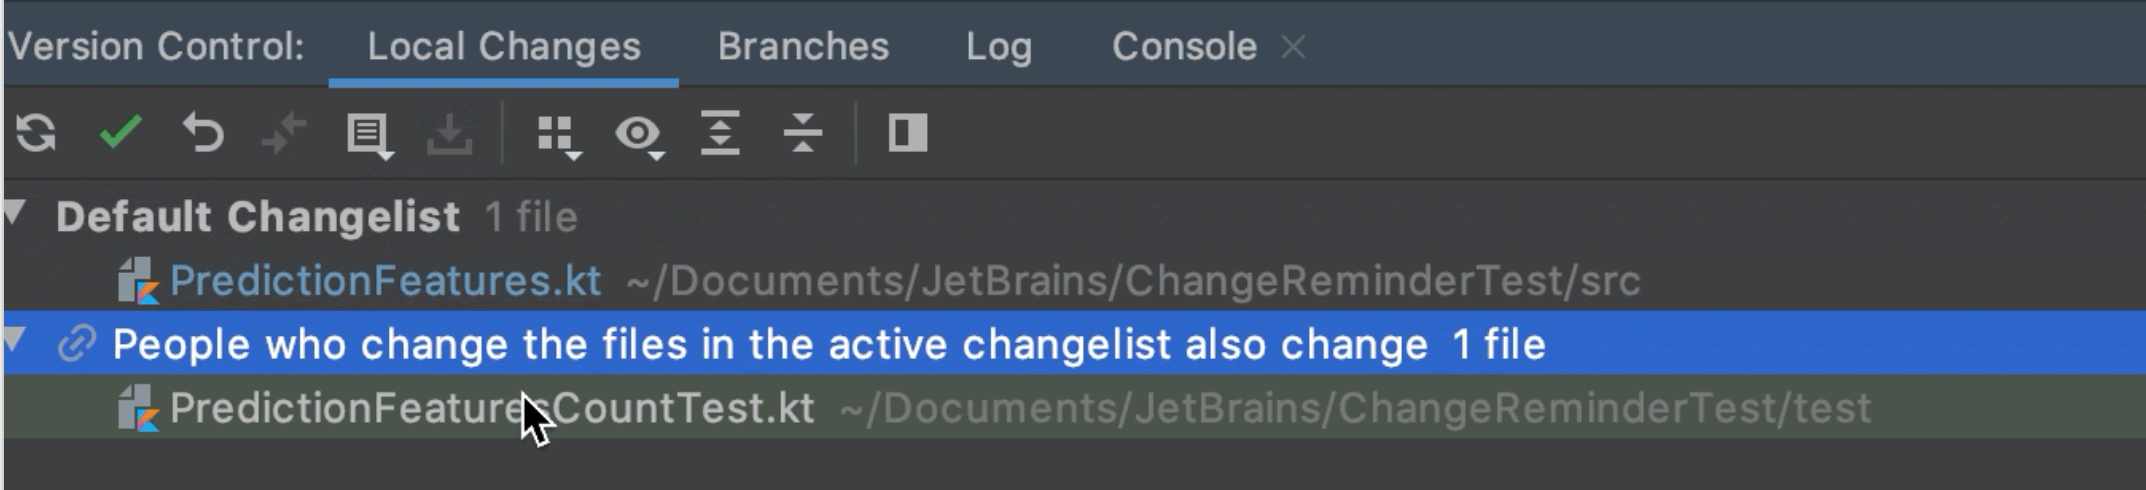
\includegraphics[scale=0.4]{ChangeReminderUI.png}
\end{figure}
Пользовательский интерфейс плагина ChangeReminder представляет из себя вершину в дереве изменений во вкладке Local Changes (см рисунок \ref{ChangeReminder-ui}). Вершина называется People who change the files in the active changelist also change. Если рекомендация составляет пустое множество файлов, то вершина становится невидимой.
\section{Практическое применение}
Плагин ChangeReminder идет в комплекте с продуктами на основе IntelliJ платформы, начиная с версии 2019.2.

%TODO
\section{Сбор статистики}\label{stats-main}
Для того, чтобы понимать, насколько хорошо работает наша решающая функция у пользователей в реальных условиях, а не на искусственно созданном наборе данных, было решено использовать сбор статистики. Также, с помощью пользовательских логов можно понять, что нужно изменить в нашей модели, чтобы число благоприятных исходов увеличилось. Для этого были записаны факторы для пар файлов, которые использовались для их для дальнейшего обучения. Не стоит забывать о том, что интерфейс плагина должен подходить пользователям. Используя статистику мы сможем понять реакцию пользователей на наши сообщения. Для этого был посчитан процент случаев, когда пользователь смотрел на предложенные файлы и когда проигнорировал нашу рекомендацию. Всего было сделано две реализации сбора пользовательской статистики. В начале статистика собиралась с использованием серверов User Logs, затем был совершен переход на более современный, встроенный в IntelliJ платформу сервис~-- Feature Usage Statistics (FUS).
\subsection{С использованием серверов User Logs}
Первая итерация сбора пользовательских логов использовала сервера внутреннего сервиса сбора статистики User Logs. Общение с User Logs серверами происходит по протоколу HTTP. Статистика пользователя для User Logs представляется в виде множества строк отчета, их формат будет изложен в секции \ref{report-line}. Отправлять пользовательские логи можно как в сжатом, так и в текстовом виде (для этого используются разные url).
\subsubsection{Модель пользовательских логов}
Пользовательские логи в User Logs представляют из себя конечный автомат. Состояние автомата~-- это данные описывающие состояние системы. А переход~-- это пользовательское действие.
\subsubsection{Строка отчета плагина}\label{report-line}
Каждая строка отчета, отправляемого в User Logs, представляет из себя части соединенные символом табуляции:
    \begin{itemize}[label={\textbullet}]
        \item $timestamp$ -- время, когда произошло пользовательское действие.
        \item $recorderId$ -- идентификатор отправителя статистики.
        \item $recoderVersion$ -- версия отправителя статистики.
        \item $userId$ -- идентификатор пользователя (создается при установке IDE).
        \item $sessionId$ -- идентификатор сессии (создается при открытии IDE).
        \item $bucket$ -- идентификатор группы (используется для A/B экспериментов).
        \item $actionType$ -- идентификатор действия пользователя.
        \item $actionJson$ -- информация о состоянии, в которое перешел пользователь.
    \end{itemize}

Рассмотрим конкретнее, какие типы действий пользователя отправлялись плагином:
    \begin{itemize}[label={\textbullet}]
        \item $COMMIT\_CLICKED$ -- нажатие кнопки Commit в Commit Dialog.
        \item $CANCEL$ -- нажатие кнопки Cancel
        \item $COMMIT$ -- нажатие кнопки Commit Anyway
    \end{itemize}

В информации о состоянии содержался $json$ в котором было несколько полей:
    \begin{itemize}[label={\textbullet}]
        \item $REPOSITORY$ -- уникальный для пользователя идентификатор репозитория.
        \item $FILES$ -- уникальные для репозитория идентификаторы файлов в коммите.
        \item $TIME$ -- время, затраченное на подсчет рекомендации.
        \item $PREDICTION$ -- уникальные для репозитория идентификаторы файлов, рекомендованные для модификации и добавления в коммит.
        \item $FACTORS$ -- факторы посчитанные для каждого рекомендованного файла.
    \end{itemize}
Идентификаторы репозитория, файлов и коммитов создает IntelliJ платформа. По данным идентификаторам нельзя идентифицировать пользователя. Таким образом, никакой приватной информации не отправляется. К тому же, при первом запуске IDE с плагином пользователю показывается нотификация о том, что плагин отправляет полностью анонимные данные для улучшения качества решающей функции.
\subsubsection{Реализация записи и отправки пользовательских логов}
\begin{figure}[!h]
\caption{Схема записи и отправки пользовательских логов}\label{jet-stat-logs}
\centering
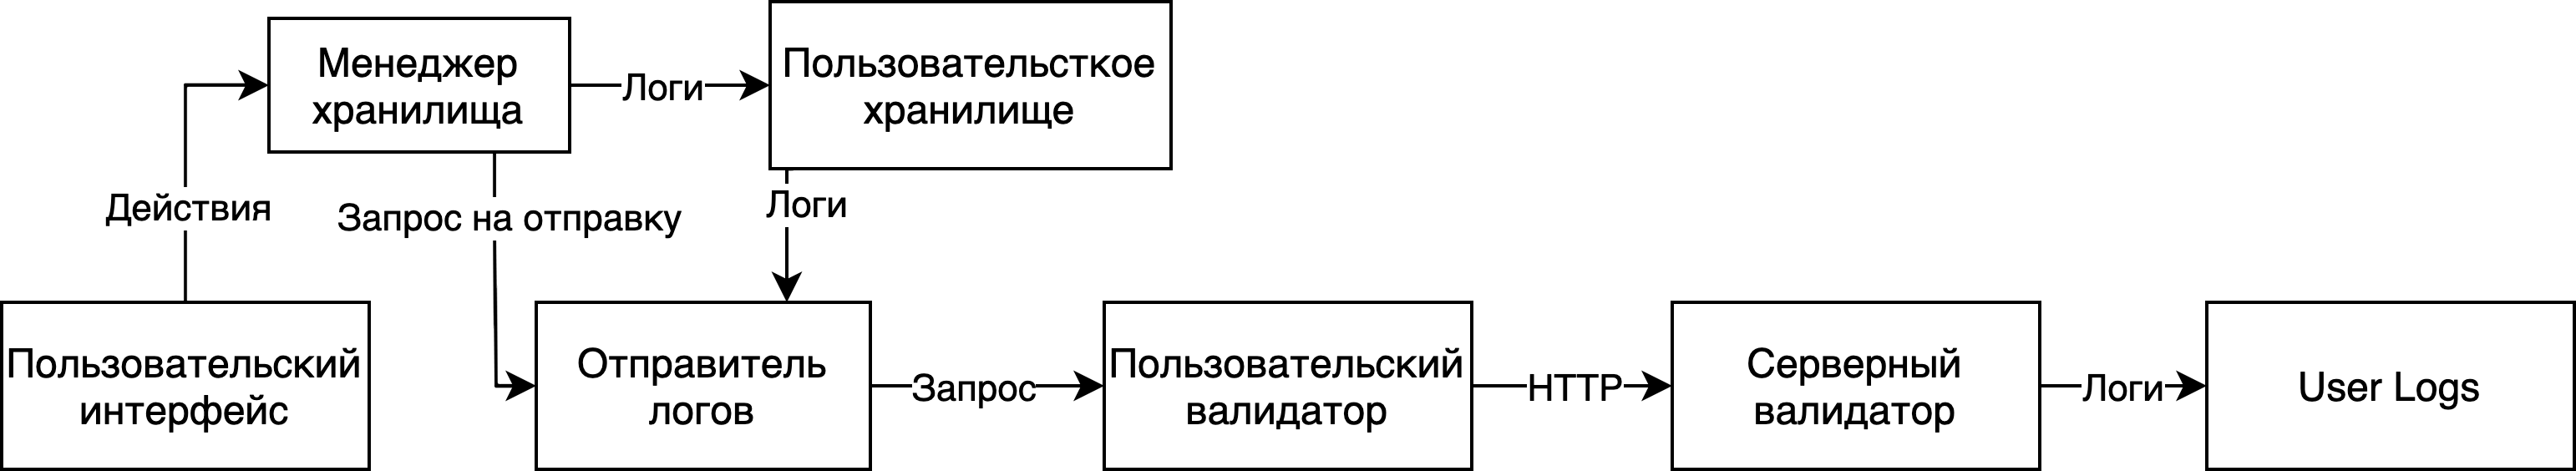
\includegraphics[scale=0.15]{User Logs.png}
\end{figure}
Реализация записи и отправки пользовательских логов показана на рисунке \ref{jet-stat-logs}. Принцип работы является достаточно популярным. При совершении пользователем какого-то действия над интерфейсом, это действие отправляется к менеджеру хранилища, который создает правильные строки отчета и сохраняет их в локальное хранилище. После этого менеджер хранилища отправляет запрос отправителю логов, чтобы сервис отправил накопившиеся данные на сервер. Если данных в локальном хранилище достаточно, то из них отправитель логов собирает HTTP запрос на сервер. Затем идет переход к одной из самых важных частей реализации~-- валидаторам. Перед тем, как отправлять данные на сервер, очень важно понять, не нарушена ли их консистентность (например, пользователю была показана рекомендация, но он ничего с ней не сделал). Для проверки консистентности данных был создан валидатор, который присутствует, как на стороне клиента, так и на стороне сервера. Только после того, как HTTP запрос прошел валидацию на клиентской стороне, он отправляется на сервер User Logs, где расположен серверный валидатор. Если пришедшие данные консистентны, то они сохраняются на сервер и ждут дальнейшей обработки.
\subsection{С использованием Feature Usage Statistics}\label{fus-main}
Следующая итерация сбора статистики плагина использовала сервис Feature Usage Statistics (FUS). FUS встроен в IntelliJ платформу.
\subsubsection{Модель пользовательских логов}
Пользовательские логи сервиса FUS представляют из себя набор событий системы. Часто, но не всегда, эти события порождаются действиями пользователя.
\subsubsection{Реализация отправки пользовательских логов}
Отправка пользовательских логов с помощью сервиса FUS является более простой, в сравнении с отправкой статистики на сервера User Logs. Feature Usage Statistics сам занимается хранением, валидацией и отправкой данных. Нашему приложению достаточно собрать $FeatureUsageData$ объект и передать его в FUS.
\chapterconclusion